% Created by tikzDevice version 0.12.3.1 on 2023-05-05 12:23:06
% !TEX encoding = UTF-8 Unicode
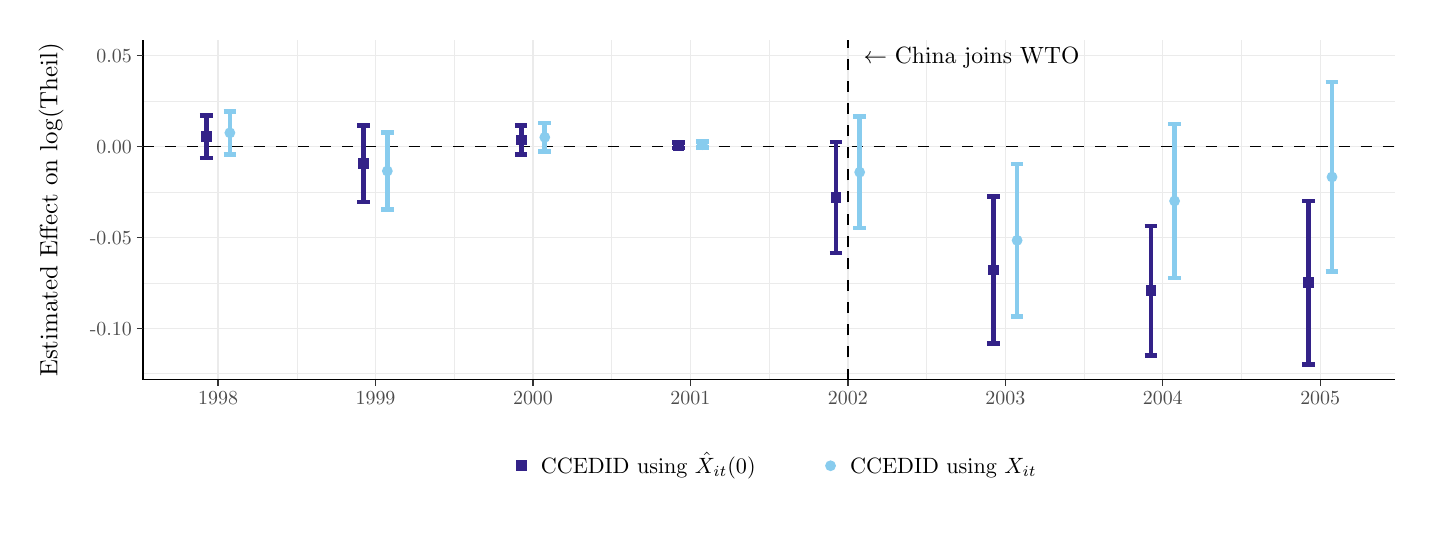
\begin{tikzpicture}[x=1pt,y=1pt]
\definecolor{fillColor}{RGB}{255,255,255}
\path[use as bounding box,fill=fillColor] (0,0) rectangle (498.66,174.53);
\begin{scope}
\path[clip] (  0.00,  0.00) rectangle (498.66,174.53);
\definecolor{drawColor}{RGB}{255,255,255}

\path[draw=drawColor,line width= 0.5pt,line join=round,line cap=round,fill=fillColor] (  0.00,  0.00) rectangle (498.66,174.53);
\end{scope}
\begin{scope}
\path[clip] ( 41.69, 47.36) rectangle (494.16,170.03);
\definecolor{fillColor}{RGB}{255,255,255}

\path[fill=fillColor] ( 41.69, 47.36) rectangle (494.16,170.03);
\definecolor{drawColor}{gray}{0.92}

\path[draw=drawColor,line width= 0.2pt,line join=round] ( 41.69, 49.50) --
	(494.16, 49.50);

\path[draw=drawColor,line width= 0.2pt,line join=round] ( 41.69, 82.34) --
	(494.16, 82.34);

\path[draw=drawColor,line width= 0.2pt,line join=round] ( 41.69,115.19) --
	(494.16,115.19);

\path[draw=drawColor,line width= 0.2pt,line join=round] ( 41.69,148.03) --
	(494.16,148.03);

\path[draw=drawColor,line width= 0.2pt,line join=round] ( 97.25, 47.36) --
	( 97.25,170.03);

\path[draw=drawColor,line width= 0.2pt,line join=round] (154.14, 47.36) --
	(154.14,170.03);

\path[draw=drawColor,line width= 0.2pt,line join=round] (211.04, 47.36) --
	(211.04,170.03);

\path[draw=drawColor,line width= 0.2pt,line join=round] (267.93, 47.36) --
	(267.93,170.03);

\path[draw=drawColor,line width= 0.2pt,line join=round] (324.82, 47.36) --
	(324.82,170.03);

\path[draw=drawColor,line width= 0.2pt,line join=round] (381.71, 47.36) --
	(381.71,170.03);

\path[draw=drawColor,line width= 0.2pt,line join=round] (438.61, 47.36) --
	(438.61,170.03);

\path[draw=drawColor,line width= 0.5pt,line join=round] ( 41.69, 65.92) --
	(494.16, 65.92);

\path[draw=drawColor,line width= 0.5pt,line join=round] ( 41.69, 98.77) --
	(494.16, 98.77);

\path[draw=drawColor,line width= 0.5pt,line join=round] ( 41.69,131.61) --
	(494.16,131.61);

\path[draw=drawColor,line width= 0.5pt,line join=round] ( 41.69,164.46) --
	(494.16,164.46);

\path[draw=drawColor,line width= 0.5pt,line join=round] ( 68.80, 47.36) --
	( 68.80,170.03);

\path[draw=drawColor,line width= 0.5pt,line join=round] (125.70, 47.36) --
	(125.70,170.03);

\path[draw=drawColor,line width= 0.5pt,line join=round] (182.59, 47.36) --
	(182.59,170.03);

\path[draw=drawColor,line width= 0.5pt,line join=round] (239.48, 47.36) --
	(239.48,170.03);

\path[draw=drawColor,line width= 0.5pt,line join=round] (296.38, 47.36) --
	(296.38,170.03);

\path[draw=drawColor,line width= 0.5pt,line join=round] (353.27, 47.36) --
	(353.27,170.03);

\path[draw=drawColor,line width= 0.5pt,line join=round] (410.16, 47.36) --
	(410.16,170.03);

\path[draw=drawColor,line width= 0.5pt,line join=round] (467.05, 47.36) --
	(467.05,170.03);
\definecolor{drawColor}{RGB}{0,0,0}

\path[draw=drawColor,line width= 0.6pt,dash pattern=on 4pt off 4pt ,line join=round] ( 41.69,131.61) -- (494.16,131.61);

\path[draw=drawColor,line width= 0.6pt,dash pattern=on 4pt off 4pt ,line join=round] (296.38, 47.36) -- (296.38,170.03);

\node[text=drawColor,anchor=base west,inner sep=0pt, outer sep=0pt, scale=  0.85] at (302.06,161.52) {$\leftarrow$ China joins WTO};
\definecolor{drawColor}{RGB}{51,34,136}

\path[draw=drawColor,line width= 1.7pt,line join=round] ( 62.26,142.74) --
	( 66.81,142.74);

\path[draw=drawColor,line width= 1.7pt,line join=round] ( 64.54,142.74) --
	( 64.54,127.44);

\path[draw=drawColor,line width= 1.7pt,line join=round] ( 62.26,127.44) --
	( 66.81,127.44);

\path[draw=drawColor,line width= 1.7pt,line join=round] (119.15,139.14) --
	(123.71,139.14);

\path[draw=drawColor,line width= 1.7pt,line join=round] (121.43,139.14) --
	(121.43,111.50);

\path[draw=drawColor,line width= 1.7pt,line join=round] (119.15,111.50) --
	(123.71,111.50);

\path[draw=drawColor,line width= 1.7pt,line join=round] (176.05,139.08) --
	(180.60,139.08);

\path[draw=drawColor,line width= 1.7pt,line join=round] (178.32,139.08) --
	(178.32,128.81);

\path[draw=drawColor,line width= 1.7pt,line join=round] (176.05,128.81) --
	(180.60,128.81);

\path[draw=drawColor,line width= 1.7pt,line join=round] (232.94,133.13) --
	(237.49,133.13);

\path[draw=drawColor,line width= 1.7pt,line join=round] (235.22,133.13) --
	(235.22,131.04);

\path[draw=drawColor,line width= 1.7pt,line join=round] (232.94,131.04) --
	(237.49,131.04);

\path[draw=drawColor,line width= 1.7pt,line join=round] (289.83,133.22) --
	(294.38,133.22);

\path[draw=drawColor,line width= 1.7pt,line join=round] (292.11,133.22) --
	(292.11, 93.13);

\path[draw=drawColor,line width= 1.7pt,line join=round] (289.83, 93.13) --
	(294.38, 93.13);

\path[draw=drawColor,line width= 1.7pt,line join=round] (346.73,113.48) --
	(351.28,113.48);

\path[draw=drawColor,line width= 1.7pt,line join=round] (349.00,113.48) --
	(349.00, 60.44);

\path[draw=drawColor,line width= 1.7pt,line join=round] (346.73, 60.44) --
	(351.28, 60.44);

\path[draw=drawColor,line width= 1.7pt,line join=round] (403.62,102.90) --
	(408.17,102.90);

\path[draw=drawColor,line width= 1.7pt,line join=round] (405.89,102.90) --
	(405.89, 56.04);

\path[draw=drawColor,line width= 1.7pt,line join=round] (403.62, 56.04) --
	(408.17, 56.04);

\path[draw=drawColor,line width= 1.7pt,line join=round] (460.51,111.93) --
	(465.06,111.93);

\path[draw=drawColor,line width= 1.7pt,line join=round] (462.79,111.93) --
	(462.79, 52.94);

\path[draw=drawColor,line width= 1.7pt,line join=round] (460.51, 52.94) --
	(465.06, 52.94);
\definecolor{drawColor}{RGB}{136,204,238}

\path[draw=drawColor,line width= 1.7pt,line join=round] ( 70.79,144.27) --
	( 75.35,144.27);

\path[draw=drawColor,line width= 1.7pt,line join=round] ( 73.07,144.27) --
	( 73.07,128.79);

\path[draw=drawColor,line width= 1.7pt,line join=round] ( 70.79,128.79) --
	( 75.35,128.79);

\path[draw=drawColor,line width= 1.7pt,line join=round] (127.69,136.72) --
	(132.24,136.72);

\path[draw=drawColor,line width= 1.7pt,line join=round] (129.96,136.72) --
	(129.96,108.73);

\path[draw=drawColor,line width= 1.7pt,line join=round] (127.69,108.73) --
	(132.24,108.73);

\path[draw=drawColor,line width= 1.7pt,line join=round] (184.58,140.11) --
	(189.13,140.11);

\path[draw=drawColor,line width= 1.7pt,line join=round] (186.86,140.11) --
	(186.86,129.71);

\path[draw=drawColor,line width= 1.7pt,line join=round] (184.58,129.71) --
	(189.13,129.71);

\path[draw=drawColor,line width= 1.7pt,line join=round] (241.47,133.33) --
	(246.02,133.33);

\path[draw=drawColor,line width= 1.7pt,line join=round] (243.75,133.33) --
	(243.75,131.23);

\path[draw=drawColor,line width= 1.7pt,line join=round] (241.47,131.23) --
	(246.02,131.23);

\path[draw=drawColor,line width= 1.7pt,line join=round] (298.37,142.45) --
	(302.92,142.45);

\path[draw=drawColor,line width= 1.7pt,line join=round] (300.64,142.45) --
	(300.64,102.15);

\path[draw=drawColor,line width= 1.7pt,line join=round] (298.37,102.15) --
	(302.92,102.15);

\path[draw=drawColor,line width= 1.7pt,line join=round] (355.26,125.26) --
	(359.81,125.26);

\path[draw=drawColor,line width= 1.7pt,line join=round] (357.53,125.26) --
	(357.53, 70.10);

\path[draw=drawColor,line width= 1.7pt,line join=round] (355.26, 70.10) --
	(359.81, 70.10);

\path[draw=drawColor,line width= 1.7pt,line join=round] (412.15,139.76) --
	(416.70,139.76);

\path[draw=drawColor,line width= 1.7pt,line join=round] (414.43,139.76) --
	(414.43, 84.03);

\path[draw=drawColor,line width= 1.7pt,line join=round] (412.15, 84.03) --
	(416.70, 84.03);

\path[draw=drawColor,line width= 1.7pt,line join=round] (469.04,154.85) --
	(473.60,154.85);

\path[draw=drawColor,line width= 1.7pt,line join=round] (471.32,154.85) --
	(471.32, 86.30);

\path[draw=drawColor,line width= 1.7pt,line join=round] (469.04, 86.30) --
	(473.60, 86.30);
\definecolor{fillColor}{RGB}{51,34,136}

\path[fill=fillColor] ( 62.57,133.13) --
	( 66.50,133.13) --
	( 66.50,137.05) --
	( 62.57,137.05) --
	cycle;

\path[fill=fillColor] (119.47,123.36) --
	(123.39,123.36) --
	(123.39,127.28) --
	(119.47,127.28) --
	cycle;

\path[fill=fillColor] (176.36,131.98) --
	(180.28,131.98) --
	(180.28,135.91) --
	(176.36,135.91) --
	cycle;

\path[fill=fillColor] (233.25,130.12) --
	(237.18,130.12) --
	(237.18,134.05) --
	(233.25,134.05) --
	cycle;

\path[fill=fillColor] (290.15,111.22) --
	(294.07,111.22) --
	(294.07,115.14) --
	(290.15,115.14) --
	cycle;

\path[fill=fillColor] (347.04, 85.00) --
	(350.96, 85.00) --
	(350.96, 88.92) --
	(347.04, 88.92) --
	cycle;

\path[fill=fillColor] (403.93, 77.51) --
	(407.86, 77.51) --
	(407.86, 81.43) --
	(403.93, 81.43) --
	cycle;

\path[fill=fillColor] (460.82, 80.47) --
	(464.75, 80.47) --
	(464.75, 84.40) --
	(460.82, 84.40) --
	cycle;
\definecolor{fillColor}{RGB}{136,204,238}

\path[fill=fillColor] ( 73.07,136.53) circle (  1.96);

\path[fill=fillColor] (129.96,122.73) circle (  1.96);

\path[fill=fillColor] (186.86,134.91) circle (  1.96);

\path[fill=fillColor] (243.75,132.28) circle (  1.96);

\path[fill=fillColor] (300.64,122.30) circle (  1.96);

\path[fill=fillColor] (357.53, 97.68) circle (  1.96);

\path[fill=fillColor] (414.43,111.90) circle (  1.96);

\path[fill=fillColor] (471.32,120.57) circle (  1.96);
\end{scope}
\begin{scope}
\path[clip] (  0.00,  0.00) rectangle (498.66,174.53);
\definecolor{drawColor}{RGB}{0,0,0}

\path[draw=drawColor,line width= 0.5pt,line join=round] ( 41.69, 47.36) --
	( 41.69,170.03);
\end{scope}
\begin{scope}
\path[clip] (  0.00,  0.00) rectangle (498.66,174.53);
\definecolor{drawColor}{gray}{0.30}

\node[text=drawColor,anchor=base east,inner sep=0pt, outer sep=0pt, scale=  0.72] at ( 37.64, 63.44) {-0.10};

\node[text=drawColor,anchor=base east,inner sep=0pt, outer sep=0pt, scale=  0.72] at ( 37.64, 96.29) {-0.05};

\node[text=drawColor,anchor=base east,inner sep=0pt, outer sep=0pt, scale=  0.72] at ( 37.64,129.13) {0.00};

\node[text=drawColor,anchor=base east,inner sep=0pt, outer sep=0pt, scale=  0.72] at ( 37.64,161.98) {0.05};
\end{scope}
\begin{scope}
\path[clip] (  0.00,  0.00) rectangle (498.66,174.53);
\definecolor{drawColor}{gray}{0.20}

\path[draw=drawColor,line width= 0.5pt,line join=round] ( 39.44, 65.92) --
	( 41.69, 65.92);

\path[draw=drawColor,line width= 0.5pt,line join=round] ( 39.44, 98.77) --
	( 41.69, 98.77);

\path[draw=drawColor,line width= 0.5pt,line join=round] ( 39.44,131.61) --
	( 41.69,131.61);

\path[draw=drawColor,line width= 0.5pt,line join=round] ( 39.44,164.46) --
	( 41.69,164.46);
\end{scope}
\begin{scope}
\path[clip] (  0.00,  0.00) rectangle (498.66,174.53);
\definecolor{drawColor}{RGB}{0,0,0}

\path[draw=drawColor,line width= 0.5pt,line join=round] ( 41.69, 47.36) --
	(494.16, 47.36);
\end{scope}
\begin{scope}
\path[clip] (  0.00,  0.00) rectangle (498.66,174.53);
\definecolor{drawColor}{gray}{0.20}

\path[draw=drawColor,line width= 0.5pt,line join=round] ( 68.80, 45.11) --
	( 68.80, 47.36);

\path[draw=drawColor,line width= 0.5pt,line join=round] (125.70, 45.11) --
	(125.70, 47.36);

\path[draw=drawColor,line width= 0.5pt,line join=round] (182.59, 45.11) --
	(182.59, 47.36);

\path[draw=drawColor,line width= 0.5pt,line join=round] (239.48, 45.11) --
	(239.48, 47.36);

\path[draw=drawColor,line width= 0.5pt,line join=round] (296.38, 45.11) --
	(296.38, 47.36);

\path[draw=drawColor,line width= 0.5pt,line join=round] (353.27, 45.11) --
	(353.27, 47.36);

\path[draw=drawColor,line width= 0.5pt,line join=round] (410.16, 45.11) --
	(410.16, 47.36);

\path[draw=drawColor,line width= 0.5pt,line join=round] (467.05, 45.11) --
	(467.05, 47.36);
\end{scope}
\begin{scope}
\path[clip] (  0.00,  0.00) rectangle (498.66,174.53);
\definecolor{drawColor}{gray}{0.30}

\node[text=drawColor,anchor=base,inner sep=0pt, outer sep=0pt, scale=  0.72] at ( 68.80, 38.35) {1998};

\node[text=drawColor,anchor=base,inner sep=0pt, outer sep=0pt, scale=  0.72] at (125.70, 38.35) {1999};

\node[text=drawColor,anchor=base,inner sep=0pt, outer sep=0pt, scale=  0.72] at (182.59, 38.35) {2000};

\node[text=drawColor,anchor=base,inner sep=0pt, outer sep=0pt, scale=  0.72] at (239.48, 38.35) {2001};

\node[text=drawColor,anchor=base,inner sep=0pt, outer sep=0pt, scale=  0.72] at (296.38, 38.35) {2002};

\node[text=drawColor,anchor=base,inner sep=0pt, outer sep=0pt, scale=  0.72] at (353.27, 38.35) {2003};

\node[text=drawColor,anchor=base,inner sep=0pt, outer sep=0pt, scale=  0.72] at (410.16, 38.35) {2004};

\node[text=drawColor,anchor=base,inner sep=0pt, outer sep=0pt, scale=  0.72] at (467.05, 38.35) {2005};
\end{scope}
\begin{scope}
\path[clip] (  0.00,  0.00) rectangle (498.66,174.53);
\definecolor{drawColor}{RGB}{0,0,0}

\node[text=drawColor,rotate= 90.00,anchor=base,inner sep=0pt, outer sep=0pt, scale=  0.90] at ( 10.70,108.70) {Estimated Effect on $\log($Theil$)$};
\end{scope}
\begin{scope}
\path[clip] (  0.00,  0.00) rectangle (498.66,174.53);
\definecolor{fillColor}{RGB}{255,255,255}

\path[fill=fillColor] (156.77,  4.50) rectangle (379.09, 27.95);
\end{scope}
\begin{scope}
\path[clip] (  0.00,  0.00) rectangle (498.66,174.53);
\definecolor{fillColor}{RGB}{255,255,255}

\path[fill=fillColor] (164.11,  9.00) rectangle (192.57, 23.45);
\end{scope}
\begin{scope}
\path[clip] (  0.00,  0.00) rectangle (498.66,174.53);
\definecolor{fillColor}{RGB}{51,34,136}

\path[fill=fillColor] (176.38, 14.26) --
	(180.30, 14.26) --
	(180.30, 18.19) --
	(176.38, 18.19) --
	cycle;
\end{scope}
\begin{scope}
\path[clip] (  0.00,  0.00) rectangle (498.66,174.53);
\definecolor{fillColor}{RGB}{255,255,255}

\path[fill=fillColor] (275.89,  9.00) rectangle (304.34, 23.45);
\end{scope}
\begin{scope}
\path[clip] (  0.00,  0.00) rectangle (498.66,174.53);
\definecolor{fillColor}{RGB}{136,204,238}

\path[fill=fillColor] (290.11, 16.23) circle (  1.96);
\end{scope}
\begin{scope}
\path[clip] (  0.00,  0.00) rectangle (498.66,174.53);
\definecolor{drawColor}{RGB}{0,0,0}

\node[text=drawColor,anchor=base west,inner sep=0pt, outer sep=0pt, scale=  0.80] at (185.41, 13.47) {CCEDID using $\hat{X}_{it}(0)$};
\end{scope}
\begin{scope}
\path[clip] (  0.00,  0.00) rectangle (498.66,174.53);
\definecolor{drawColor}{RGB}{0,0,0}

\node[text=drawColor,anchor=base west,inner sep=0pt, outer sep=0pt, scale=  0.80] at (297.18, 13.47) {CCEDID using $X_{it}$};
\end{scope}
\end{tikzpicture}
